\documentclass[10pt]{article}
\usepackage[utf8]{inputenc}

\title{Granular Dynamic Stochastic Synthesis on the VCV Rack platform}
\author{Samuel Laing}
\date{May 2019}

\usepackage{natbib}
\usepackage{graphicx}

\usepackage[utf8]{inputenc}
\usepackage[TS1,T1]{fontenc}
\usepackage{fourier, heuristica}
\usepackage{array, booktabs}
\usepackage{graphicx}
\usepackage[x11names,table]{xcolor}
\usepackage{caption}

\usepackage[margin=1.5in]{geometry}
\usepackage{algorithm, algorithmic}

\DeclareCaptionFont{blue}{\color{LightSteelBlue3}}

\newcommand{\foo}{\color{LightSteelBlue3}\makebox[0pt]{\textbullet}\hskip-0.5pt\vrule width 1pt\hspace{\labelsep}}


\begin{document}

\maketitle
\begin{abstract}
The goal of digital sound synthesis processes is often sonic complexity - to imitate that which is inherent in natural sounds - while being efficient enough for real-time sound generation. Frequency modulated (FM) synthesis, for instance, accomplishes complexity through the generation of sidebands at frequencies corresponding to the carrier and modulator frequencies. This project focuses on a non-standard, microsound synthesis method, stochastic synthesis, which uses random walks to produce complex, time-varying waves, and presents a novel extension to the synthesis process, as well an implementation as a plugin for the VCV Rack platform. Iannis Xenakis first implemented Dynamic Stochastic Synthesis in 1971 with his GENDY1 program. The synthesis method directly produces and then manipulates a novel waveform using stochastic processes. This project presents an extension to the DSS method through the addition of an underlying synchronous granular synthesis process that informs the interpolation of the stochastic waveform. The granular process granulates sine waves and FM sine waves according random walks. The resulting form of sound synthesis, Granular Dynamic Stochastic synthesis, maintains much of the sonic character of stochastic synthesis, while expanding its sonic range and complexity. Two more extensions are presented and implemented as VCV Rack modules: a generator module performing stochastic concatenation of GDSS generated waveforms, and an effects module that uses similar stochastic methods to continually morph a supplied signal.
\end{abstract}

\pagebreak
\section{Background}
The composer and early computer musician Iannis Xenakis drew heavily upon stochastic processes in the development of his unique musical styles and experiments. Xenakis often used stochastic processes and distributions to map the placement of musical events over time and the frequency spectrum. For instance, in his piece \textit{Pithopraktra}, Xenakis arranges in time and pitch sharp glissandi of 46 string instruments according to Gaussian and Poisson distributions.\citep{xenakis1992} Additionally, in \textit{Analogique A} and \textit{Analogique B} sonic screens with events stochastically distributed throughout are used to shape the tonality and movement of the piece. 

In each of these pieces, stochastic processes are embedded in the macro controls shaping the density of a cloud, or the sparsity of a section. Xenakis's development of stochastic synthesis moved the stochastic process away from the macro, as it is used to inform a type of microsound synthesis. Microsound synthesis entails the direct manipulation and control of a waveform. Another computer musician pioneering non-standard synthesis techniques, Herbert Brun, with the technical assistance of Gary Grossman, composed using SAWDUST, a synthesis tool that allowed Brun to "work with the smallest parts of waveforms, to link them and to mingle or merge them with one another."\citep{sergio2006} SAWDUST was, however, a largely deterministic process, and did not embrace the power of stochastic processes like Xenakis's attempt at microsound synthesis.

\subsection{Dynamic Stochastic Synthesis}
Xenakis implemented Dynamic Stochastic Synthesis (DSS) in his 1971 GENDY1 program written in the BASIC programming language with the help of Marie-Helene Serra.\citep{xenakis1992} DSS directly synthesises a wave by the linear interpolation of breakpoints. Breakpoints are an important concept at the core of Xenakis's non-standard micro-sound synthesis method. Each breakpoint represents a point, an amplitude and a duration value, in the to-be produced wave. After each cycle, each breakpoint takes a step where its amplitude and duration values are altered by a random walk. So, the wave being produced will continually morph and step its way through sonic space, bringing in and taking out numerous complicated transients in the process. It is the small increment walks of each breakpoint that gives stochastic synthesis its unique and complex sonic character.



\subsection{Existing Implementations and Extensions}
Since Xenakis first introduced DSS there have been several attempts to extend the method of synthesis. Nick Collins adapted Xenakis's DSS to the SuperCollider3 platform with his Gendy1, Gendy2, and Gendy3 UGens. (TODO CITE UGENS) While these implemenations do not extend the method of synthesis, they do expose it to a greater user base on the SC3 platform. Luc Dobereiner's PHINGEN, or Physically Informed Stochastic Synthesis, is a novel extension to DSS synthesis by replacing the linear interpolation between breakpoints with a physical model.\citep{luc2011dobereiner} PHINGEN is also available on the SuperCollider3 platform as a UGen.

\section{Extending Dynamic Stochastic Synthesis}
To extend Xenakis's stochastic synthesis, I incorporated another synthesis type: granular synthesis. DSS generally utilizes linear interpolation to calculate samples in-between breakpoints. If a small number of breakpoints is used this can limit the complexity of produced sounds. By incorporating a synchronous granular synthesis method into the interpolation process, I have introduced the ability to add micro-variations to the DSS wave. 

The incorporation of granular synthesis into stochastic synthesis begins with the expansion of the breakpoint. For stochastic synthesis, the breakpoint represents only amplitude and duration values. Grain offset, grain rate, and grain amplitude values are added to each breakpoint in order to inform the granular synthesis. Granular synthesis requires a sonic resource or raw material that is to be enveloped. To avoid the added complexity of sample storage, or input signal granulation, GDSS uses sine waves, or single-carrier single-modulator FM sine waves, as the sonic material. Lines (TODO pseudocode of algorithm) shows the different processes that sine waves versus FM sine waves granulation require.

\begin{algorithm}\captionsetup{labelfont={sc,bf}, labelsep=newline}
\caption{Granular Dynamic Stochastic Synthesis Algorithm}
    \begin{algorithmic}
        \STATE $bpts\gets [\{amp,\ dur,\ off,\ grate\}]$
        \STATE $bpt\gets bpts[0]$
        \STATE $bpt\_next\gets None$
        \STATE $index\gets 0$
        \STATE $prob\_dist\gets UNIFORM$
        \LOOP
            \IF{$phase >= 1.0$}
                \STATE index++\\
                \STATE $bpts[index].amp += rand(prob\_dist)$
                \STATE $bpts[index].dur += rand(prob\_dist)$
                \STATE $bpts[index].off += rand(prob\_dist)$
                \STATE $bpts[index].grate += rand(prob\_dist)$
                \STATE $bpt\gets bpt\_next$\\
                \STATE $bpt\_next\gets bpts[index]$
            \ENDIF
            \STATE $amp\gets bpt.amp + (env * sinf(bpt.off))$
            \STATE $amp\_next\gets bpt\_next.amp + (env\_next * sinf(bpt\_next.off))$
            \STATE $amp\_out\gets ((1.0 - phase) * amp) + (phase * amp\_next)$
            \STATE $speed\gets freq * bpts.size$
            \STATE $speed += phase$
            \STATE $emit()$
        \ENDLOOP
    \end{algorithmic}
\end{algorithm}

\subsection{Stochastic Concatenation}
Sergio Luque, in \textit{Stochastic Synthesis: Origins and Extensions}, presents the method of stochastic concatenation, as an extension of Xenakis's original stochastic synthesis.\citep{sergio2006} The process does not alter the core method of stochastic synthesis, but presents stochastic concatenation, which entails multiple stochastic synthesis generators producing waves that are concatenated one after another to form new output wave. 

\subsection{The Stochastic Method as Effect}
DSS and now GDSS are both generative processes using random walks to continually alter the produced sound. The same stochastic process can, instead, be used as means for sonic effect through application to an existing waveform. I present a method of morphing a sampled waveform using the random walks of breakpoints. Each breakpoint still represents an amplitude and duration value, but now they correspond to the length and amplitude of an envelope, which is to be applied to a section of the sample wave. (TODO pseudocode)

\begin{algorithm}\captionsetup{labelfont={sc,bf}, labelsep=newline}
\caption{Stochastic Effect Algorithm}
    \begin{algorithmic}
        \STATE $bpts\gets [\{amp,\ dur\}]$
        \STATE $bpt\gets bpts[0]$
        \STATE $bpt\_next\gets None$
        \STATE $index\gets 0$
        \STATE $prob\_dist\gets UNIFORM$
        \STATE $sample\gets [float]$
        \LOOP
            \IF{$phase >= 1.0$}
                \STATE index++\\
            \ENDIF
            \STATE $emit()$
        \ENDLOOP
    \end{algorithmic}
\end{algorithm}

\subsection{Goals}
The goal of extending DSS in both method and in implementation is to one expand upon the tonal and timbral range of the synthesis and to expand usage of non-standard synthesis methods to a new musical platform. 

\section{Implementation and Modules}
There are many existing platforms and technologies for the development of DSP plugins: Will Perkle's RackAFX, SuperCollider3, (find more).\citep{rackafx} I chose to use a new platform, VCV Rack, which simulates modular synth hardware. VCV Rack is a fully open-source program that was started in 2016 by Andrew Belt, and has recently gained popularity in the world of music-software technology.\citep{vcvrack} Unlike the SuperCollider3 UGen interface, samples in VCV Rack are not generated in blocks, rather each sample is generated individually. While this method of sample generation is less efficient, and less easily parallelized, it is more adherent to the modular synth paradigm.

\subsection{VCV Rack Plugin Development}

VCV Rack facilitates the development of new modules, or plugins, for the platform by exposing the \texttt{Model} class, which accepts \texttt{Module} and \texttt{ModuleWidget} structs. The \texttt{Module} struct is response for the plugins logic. The Rack engine calls \texttt{Module.step()} during each cycle. The \texttt{ModuleWidget} handles the UI for the module and specifies the type and location of controls for the panel. Each of the modules described below was implemented by extending the \texttt{Module} and \texttt{ModuleWidget} \texttt{structs} to create a new \texttt{Model}. All together, the modules are released as a package to the VCV Rack community under the name \texttt{StochKit}, short for Stochastic Toolkit.

\subsection{GRANDY}
The main module of the stochastic suite is the GRANDY module. GRANDY is a generator module that implements Granular Dynamic Stochastic Synthesis. Most parameters are exposed through knobs for the user to control. The module is modelled off of other voltage controlled oscillator (VCO) modules, so there is a knob to control the frequency of the produced wave, and the ability to modulate this set frequency through CV. 

\subsubsection{Controls}
The two top-most nobs, \texttt{freq} and \texttt{bpts}, both may be used to control the pitch of the outcoming wave. The \texttt{freq} control is more predictable as it directly reduces the distance between each breakpoint to alter the pitch. The \texttt{bpts} control, however, alters the number of breakpoints that are used in the synthesis, consequently any change in the number of breakpoints causes a change in the length of a wave cycle and a change in pitch. The two knobs below, \texttt{astp} and \texttt{dstp}, control the maximum step an amplitude value and duration value may take during their respective random walks. Increasing the \texttt{astp} parameter causes the timbre of the produced sound to change more rapidly, as transients fade in and out. While increasing the \texttt{dstp} parameter causes duration values to vary more rapidly leading to a wave that oscillates around several main frequencies, never settling for long, since the wavelength is quickly changing. Each of these controls has accompanying inputs for control by CV and corresponding knobs for the attenuation of the input signals. Controls without CV inputs are the \texttt{pdst} switch, which toggles the used probability distribution between Uniform, Cauchy, and Arcsin distributions and the \texttt{mirr} switch that toggles between mirroring and wrapping at random walk bounds.

\subsubsection{Granular Controls}
There are two sets of control for the granular aspects of the GRANDY module. The user is able to toggle between sine wave or fm sine wave granular synthesis with a switch. Controls for the frequency sine wave granular synthesis are located above the divided line. The frequency of the sine wave is controllable by the \texttt{gfreq} knob and the corresponding CV input. The controls for fm sine waves, below the dividing line, entail knobs for the frequency of the carrier and modulator waves, and a knob for the index of modulation. 

\begin{figure}
  \caption{The VCV Rack Grandy module.}
  \centering
    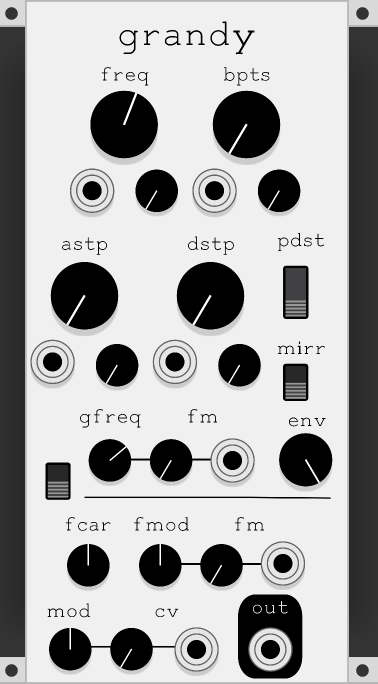
\includegraphics[height=0.25\textheight]{grandy}
\end{figure}

\subsection{STITCHER}
The STITCHER implements stochastic contatenation, as described by Luque, uses GRANDY instead of GENDYN generators. Each oscillator can be controlled separately, or by a set of global parameter knobs. The wave output by the module is a successive concatenation of waves output by each of the GRANDY oscillators.

Luque describes the concatenation of stochastic waves as being another stochastically determined process, 'using tendency masks, or ...' (TODO).\citep{sergio2006} My implementation, instead, allows the user/musician control over this process. The number of wave cycles a single oscillator outputs before the next oscillator is used, and whether an oscillator is active in the synthesis at a given time are both parameters the user may control using the corresponding knobs.

\subsubsection{Local Controls}

\subsubsection{Global Controls}

\begin{figure}
  \caption{The VCV Rack Stitcher module.}
  \centering
    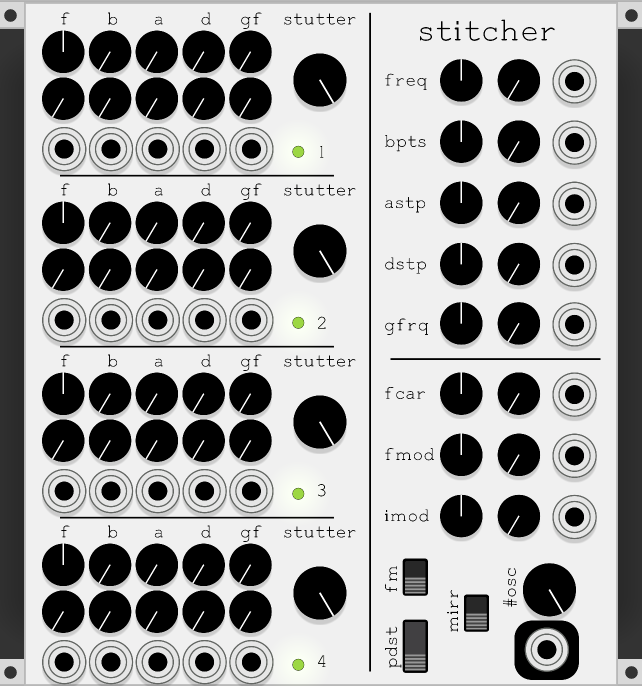
\includegraphics[height=0.25\textheight]{stitcher}
\end{figure}

\subsection{GenECHO}
The GenECHO, unlike the GRANDY and STITCHER modules, is not a generater, rather it is an effects module. On a gate input, the module samples an input signal and proceeds to apply a 'stochastic decomposition' to the sampled wave. GenECHO, like GRANDY, maintains a number of breakpoints. The number of breakpoints is influenced by the length of the sample being 'echoed' and a controllable breakpoint-spacing parameter. As the wave is repeatedly looped through, each breakpoint applies an envelope with a stochastically-generated amplitude to the stored sample. Over time the stored sample is increasingly morphed by the stochastic shifts causing new sounds to appear.

\subsubsection{Controls}
The section in the top left of GenECHO's panel handles the capturing of an input signal for effect application. The \texttt{l} knob effects the length of sample and the \texttt{i} input read in the sample upon receiving a gate to the \texttt{g} input.

\begin{figure}
  \caption{The VCV Rack GenEcho module.}
  \centering
    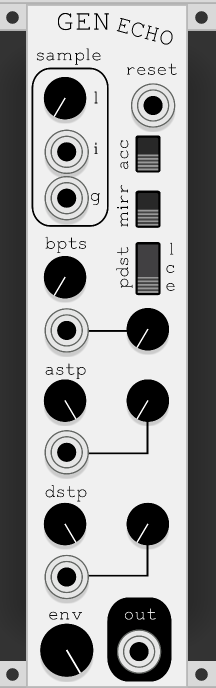
\includegraphics[height=0.25\textheight]{genecho}
\end{figure}

\section{Results}
The completed modules are available for download and use with the VCV Rack Platform. The GRANDY oscillator demonstrates Granular Dynamic Stochastic Synthesis's ability to produce a wide range of complex sounds, both those that sounds similar to those produce by GENDYN and beyond. The adaptation of stochastic synthesis methods to the VCV Rack platform was largely successful, and opens up a wide range of sonic and aesthetic possibilities to those using the VCV Rack platform. 

\section{Future Directions}
STITCHER could be extended to incorporate more of the ideas presented by Luque regarding the selection of active oscillator.


\section{Acknowledgements}

\pagebreak
\bibliographystyle{plain}
\bibliography{references}

\end{document}
